%!TEX root = main.tex

\title{The \texttt{tugPoster} Package}
\author{Markus Quaritsch}

\begin{document}
	\maketitle

	\tableofcontents

\section{Introduction}

The intention of this \LaTeX class is on the one hand to greatly simplify the process of creating posters and on the other hand to produce nice-looking posters that follow the TU Graz design guidelines. The \tugPoster{} class makes among others heavy use of the  \LaTeX{} packages \texttt{tcolorbox}, \texttt{tikz} and \texttt{enumitem}. 

This document describes the options, commands, and environments defined within the \tugPoster{} class and how you can use them to create a poster. All commands defined by \tugPoster{} use the prefix \texttt{IPT}.

% used packages, purpose
% prefix

\section{Creating a Poster}

\subsection{Minimal Working Example}

To start with creating a new poster we use the following code:

%----------------------------------------------------------
\texLstInputSampleFull{lst:mwe}{Minimal Working Example}{src/1_poster_mwe}
%----------------------------------------------------------

The \LaTeX code in \Cref{lst:mwe} should produce a PDF document of size A0 (841\,mm $\times$ 1189\,mm) with the main layout elements (i.e., the institute's short name on the left, the TU Graz logo and claim on top and the institute name and address, etc.)

\subsection{Adjusting Poster Size}

The \tugPoster{} package supports different paper sizes for the poster. To select a certain size simply add the option \texttt{size=} followed by a supported poster size to the document class options. The supported poster sizes are listed in \Cref{sec:reference}

%----------------------------------------------------------
\texLstInputSample{lst:size}{Adding authors}{src/1b_size}{1}{2}
%----------------------------------------------------------


%-------------------------------------------------------------------------
\subsection{Author, Affiliation, Email Addresses}

The authors can be typeset either in one column or if necessary in two columns. Therefore, the commands \texttt{\bs{}authorName$<$A/B$>$}, \texttt{\bs{}authorAffiliation$<$A/B$>$}, and \texttt{\bs{}authorEmail$<$A/B$>$} can be used. Contents of the commands with the suffix \texttt{A} are put on the left column while the others are placed on the right column. If only the commands with suffix \texttt{A} are used then the authors can span the whole page width (see \Cref{lst:authors}).

%----------------------------------------------------------
\texLstInputSample{lst:authors}{Adding authors}{src/2_authors}{14}{20}
%----------------------------------------------------------


%-------------------------------------------------------------------------
\subsection{Footer} % (fold)
\label{subsed:footer}

In the footer there is some space reserved for partner and/or sponsor logos. In addition there is a QR-code that points to a landing-page on the institute's website.

By default the QR-code points to the institute's website. In case the QR-code shall point to a landing page or a more specific sub-page (e.g., project page), you can add this as optional first argument to \texttt{\bs{}IPTInstituteUrl}.  Please make sure to use the correct URL and that the QR-code points to the correct web page (cf. \Cref{lst:qrcode}).
The QR-code can also be omitted using the statement \texttt{\bs{}NoQRCode} (cf: \Cref{lst:noqrcode}). You can also place an NFC tag behind the poster with some additional information or data. This can be indicated by an according logo using the statement \texttt{\bs{}ShowNFC} (cf. \Cref{lst:nfc}).


%----------------------------------------------------------
\texLstInputSample{lst:qrcode}{Adapting QR-Code target URL}{src/3_qr-code}{8}{10}
%----------------------------------------------------------

%----------------------------------------------------------
\texLstInputSample{lst:noqrcode}{Omitting the QR-Code}{src/4_no_qr-code}{9}{11}
%----------------------------------------------------------

%----------------------------------------------------------
\texLstInputSample{lst:nfc}{Showing the NFC icon}{src/5_nfc-logo}{9}{11}
%----------------------------------------------------------

For adding partner and/or sponsor logos to the footer, the command \texttt{\bs{}IPTpartner} is provided. Using this command an arbitrary number of partner-logos can be added in the footer. This command has to come before \texttt{\bs{}begin\{document\}}. The logos are vertically aligned and horizontally distributed and limited to a maximum height. If you need to adjust individual logos (e.g., make it smaller), you can provide the optional argument \texttt{imgoptions}:] which contains options for the the \texttt{\bs{}includegraphics} command.

An additional note can be placed at the top of the footer with the \texttt{\bs{}IPTpartnersNote} command.

%----------------------------------------------------------
\texLstInputSample{lst:parnterlogos}{Partner logos in the footer}{src/6_partner-logos}{20}{24}
%----------------------------------------------------------


\subsubsection{Advanced Footer Layout}

In case you want to add further content or have special placement constraints an alternative command \texttt{\bs{}IPTpartners} is provided. The argument given to this command is placed in a minipage so you can add arbitrary contents. 

\Cref{lst:customFooter} shows an example how a number of images with different height can be vertically aligned to the center (note: for demonstration purpose a simple \texttt{\bs{}framebox} is used in the example. You can replace this with an \texttt{\bs{}includegraphics} command).
In addition a single line of text can be added to the footer using the command \texttt{\bs{}IPTpartnersNote} mentioning funding contracts etc.

%----------------------------------------------------------
\texLstInputSample{lst:customFooter}{Custom footer layout}{src/7_custom-footer}{20}{27}
%----------------------------------------------------------



%-------------------------------------------------------------------------
\subsection{Main Content} % (fold)

The main content is composed of several content blocks. Every content block has a title and some content. The title is set in a blue large bold font and has a rule below indicating the width of the content block.

The content blocks can either span the whole page width or can be placed in the left or right columns. It is not necessary that the whole poster is either single column or two columns. This can be mixed as necessary and as the content allows.

A basic content block is added by using the environment \texttt{IPTblock} (see \Cref{lst:iptblock}). The mandatory argument is the title of the content block. By default, the content block spans the whole page width and the content inside the content block is typeset in a single column.

%----------------------------------------------------------
\texLstInputSample{lst:iptblock}{Basic Content Block}{src/8_main-content_iptblock}{27}{33}
%----------------------------------------------------------

If you want to place two content blocks next to each other (i.e., use a two-column layout) you have to use the environment \texttt{IPTtwocol} (see \Cref{lst:iptlayouttwocol}). Inside the environment is the content for the left column, followed by the command \texttt{\bs{}IPTcolbreak} and then the content for the right column. The content for both columns is usually a \texttt{IPTblock} content block. Of course, you can have more than one \texttt{IPTblock} in every column.

%----------------------------------------------------------
\texLstInputSample{lst:iptlayouttwocol}{Two-column layout}{src/9_main-content_twocol}{32}{44}
%----------------------------------------------------------


The content within a content block can either be a single column or two columns. The easy way to typeset the content in two columns is to simply add the option \texttt{twocol} to the \texttt{IPTblock} environment (see \Cref{lst:iptcontenttwocol})

%----------------------------------------------------------
\texLstInputSample{lst:iptcontenttwocol}{Content block with two columns}{src/10_main-content_contenttwocol}{32}{36}
%----------------------------------------------------------


Another way to typeset the content within a content block in two columns is to use the \texttt{IPTcols} environment. This environment produces a smaller gap between columns and should therefore \textbf{not} be used to separate columns at the first level but either to further split the content of the left or right column. On the top-level you can use \textbf{IPTtwocol} within a content block spanning the whole page width. \texttt{IPTcols} is more flexible concerning the subdivision of the columns. As mandatory argument you have to specify the width of the left column (between 0.0 and 1.0). This allows to have an image next to some text and use more space for the image or the text, depending on the situation. Obviously, after the \texttt{IPTcols} environment you can place further content which spans both columns (see \Cref{lst:iptcontenttwocol2}). 

%----------------------------------------------------------
\texLstInputSample{lst:iptcontenttwocol2}{Nested two-column layout}{src/11_main-content_nestedtwocol}{32}{40}
%----------------------------------------------------------

For more complex layouts it is often the case that you need to place a figure next to some text and another figure below spans both columns, etc. In such cases it is necessary (and intended) to arbitrarily nest the above described environments \texttt{IPTblock}, \texttt{IPTtwocol}, and \texttt{IPTcols}.


%-------------------------------------------------------------------------
\subsubsection{Subheader, Subsubheader} % (fold)
\label{ssub:subheader_subsubheader}

Within the content blocks you can add further headlines, i.e., subheader and subsubheader. Therefore, dedicated commands are available: \texttt{\bs{}IPTsection} and \texttt{\bs{}IPTsubsection} (see \Cref{lst:iptsection}).

%----------------------------------------------------------
\texLstInputSample{lst:iptsection}{Subheader, Subsubheader}{src/12_main-content_subheader}{32}{40}
%----------------------------------------------------------

% subsubsection subheader_subsubheader (end)

\subsection{Bullet Lists}

Bullet lists can be used as in every \LaTeX document via the \texttt{itemize} environment. Via the \texttt{enumitem} package the layout of the lists has been adapted to match the intended style. Up to three itemized lists can be nested (see \Cref{lst:itemize}).

%----------------------------------------------------------
\texLstInputSample{lst:itemize}{Bullet Lists}{src/13_main-content_itemize}{32}{45}
%----------------------------------------------------------


\subsection{Figures}

Adding figures to a latex document and placing them at a certain position is always cumbersome in \LaTeX documents. Hence, we provide a new command \texttt{\bs{IPTgraphics}} that allows to easily add figures at a certain position. 
\texttt{IPTgraphics} takes an optional argument with of key-value options as described below and a mandatory argument of the file name to include.

\texttt{IPTgraphics} supports the following arguments:
\begin{description}
	\item[\texttt{imgoptions}:] this is a list of options that is directly passed to the \texttt{\bs{}includegraphics} command. here you can adjust the size of the image, rotate or crop the image, etc.
	\item[\texttt{caption}:] here you can specify the caption which is typeset below the image
	\item[\texttt{label}:] allows to define a label for the figure that can be used in a \texttt{\bs{}ref} command
\end{description}

The content block added via \texttt{IPTgraphics} always spans the current maximum text width/column width. If you want to use more or less space for the image you need to adjust the text width (i.e. the column width). As option for the \texttt{includegraphics} command you can use \texttt{\bs{}textwidth} which is the current width of the content block.

%----------------------------------------------------------
\texLstInputSample{lst:graphics}{Adding Images}{src/14_main-content_figures}{35}{39}
%----------------------------------------------------------

\subsection{Abstract}

In case you want to add a short abstract to the poster, \tugPoster{} provides a dedicated content block for this because the text of the abstract is slightly smaller and the the text is justified. To add an abstract simply use the environment \texttt{IPTabstractblock} similar to the previously explained \texttt{IPTblock}. \texttt{IPTabstractblock} does not support two-column text and should therefore be only used spanning one column of the whole poster.

%----------------------------------------------------------
\texLstInputSample{lst:abstract}{Abstract block}{src/15_main-content_abstract}{33}{35}
%----------------------------------------------------------


\subsection{References}

Adding references to the poster requires two steps. First you need to add a content block using the \texttt{IPTrefsblock} environment. Similar to the abstract content block the references content block does not support the \texttt{twocolumn} option. The references block can be used either in a single column or spanning both columns.

Second, inside the \texttt{IPTrefsblock} use the environment \texttt{refs} to add your references. Every reference is a single \texttt{\bs{}item} inside the \texttt{refs} environment. 

The contents of the references are automatically typeset in either two or three columns, depending on the width of the references block.

%----------------------------------------------------------
\texLstInputSample{lst:references}{Nested two-column layout}{src/16_main-content_references}{35}{44}
%----------------------------------------------------------

\subsection{Advanced Layouts}

\subsubsection{Relative Lengths}

The \tugPoster{} class supports different papaer sizes. Depending on the paper size, the font size and all other layout elements (header, footer, etc.) adjusted. In case you want to prepare your poster for different paper sizes and it is not sufficient to rely on measures such as \texttt{\bs{}textwidth}, additional lengths are provided:

\begin{description}
	\item[\texttt{IPTRelWidth}:] 1~\% of the final page width, i.e. 8.41\,mm for A0 or 5.94\,mm for A1
	\item[\texttt{IPTRelHeight}:] 1~\% of the final page height, i.e. 11.89\,mm for A0 or 8.41\,mm for A1
\end{description}

This can be helpful for adjusting the size of images, etc., (see for example \Cref{lst:iptcontentthreecol})

\subsubsection{Three Column Content}

A special content block is the \texttt{\bs{}IPTcolorBlock3}. This content block provides three columns, each in its own minipage. Every column can be underlaid with some background color and between the header and the content every column can display an image. All three columns are of equal height and all three images are of equal height (and cropped in order to fill the available space).

\texttt{IPTcolorBlock3} supports the following arguments:
\begin{description}
	\item[\texttt{color1}/\texttt{color2}/\texttt{color3}:] defines the background color for the three columns
	\item[\texttt{image1}/\texttt{image2}/\texttt{image3}:] defines the image placed on top of every column
	\item[\texttt{imageHeight}:] defines the height of the images (if used)
\end{description}

%----------------------------------------------------------
\texLstInputSample{lst:iptcontentthreecol}{Content block with thee columns}{src/17_main-content_3cols}{43}{61}
%----------------------------------------------------------

\subsubsection{Custom Instute Banner}

In case you want to place a custom banner on the left-hand side of the poster instead of the institute's abbreviation the command \texttt{\bs{IPTInstituteBanner}} allows to place picture instead. If this command is used, the institute's short name is ignored.

%----------------------------------------------------------
\texLstInputSample{lst:iptcustombanner}{Custom Banner}{src/18_main-content_custom-banner}{19}{21}
%----------------------------------------------------------

\subsubsection{Customizing Colors}

The colors of the block headers and the color of the rectangle on the left-hand side above the institute's abbreviation can be customized with the commands \texttt{\bs{IPTHeaderColor}} and \texttt{\bs{IPTInstituteColor}}, see \Cref{lst:colors}

%----------------------------------------------------------
\texLstInputSample{lst:colors}{Custom Banner}{src/19_colors}{29}{32}
%----------------------------------------------------------


\subsection{Preparing for Print}

If your printer does not support cuting the poster to the exact size or the printer leaves a certain margin around the poster, you can add either crop marks or a crop rectangle to the poster. This can be achieved by either adding the option \texttt{cropmarks} or \texttt{croprectangle} as documentclass option. If you add one of those options, also some meta-information such as the \LaTeX jobname, compilation date, etc., is added at the bleed.

The option \texttt{cropmarks} adds short lines slightly outside the final paper size while \texttt{croprectangle} additionally adds a thin rectangle at the page margins (see \Cref{fig:cropmarks}.

\section{Summary of Commands/Environments/Options}
\label{sec:reference}

\begin{description}
	\item[Document Class Options:]~
		\begin{itemize}
			\item \texttt{debug}: enables the debugging feature and highlights the bounding boxes of the content elements in different colors (see \Cref{sec:debugging})
			\item \texttt{cropmarks}: produces a PDF that includes crop marks (and color bars) for cropping the printed poster
			\item \texttt{croprectangle}: same as cropmarks but with an additional rectangle at the poster's margins
			\item \texttt{size}: select the size of the poster. Currently \texttt{A0} (default), \texttt{A1}, and \texttt{70x100} are supported
		\end{itemize}
	\item[\texttt{IPTpartnersNote}:]
		Adds a note to the footer. Typically used to give credits to sponsors and partners involved.
	\item[\texttt{IPTpartner}:]
		Adds the logo of a partner to the footer. This command can be used multiple times
	\item[\texttt{IPTpartners}:]
		Alternative to \texttt{\bs{}IPTpartner} if some special content needs to be added to the footer. (see \Cref{subsed:footer})
	
	\item[\texttt{IPTHeaderColor}:] Changes the color of all block headers. Needs to be defined via \texttt{\bs{}definecolor}, see \Cref{lst:colors}

	\item[\texttt{IPTInstituteColor}:] Changes the color of rectangle on the left banner. Needs to be defined via \texttt{\bs{}definecolor}, see \Cref{lst:colors}. Not used if \texttt{IPTInstituteBanner} is set.

	\item[\texttt{IPTInstituteName}:] Full name of the institute, printed at the poster's header.

	\item[\texttt{IPTInstituteAddress}:] Full address of the institute, printed at the poster's header.

	\item[\texttt{IPTInstituteEmail}:] General contact e-mail address, printed at the poster's header.

	\item[\texttt{IPTInstituteShort}:] Abbreviation of the institute. printed at the banner on the left side. Not used if \texttt{IPTInstituteBanner} is set.

	\item[\texttt{IPTInstituteBanner}:] Use a custom picture as banner on the left side.

	\item[\texttt{IPTInstituteURL}:] Short URL of the institute's website. printed next to the QR-code in the footer. A full link to sub-page of the website can be specified via the optional first argument. Not used if \texttt{\bs{}NoQRCode} is used.

	\item[\texttt{NoQRCode}:] Do not print the QR-code pointing to the institute's website in the footer

	\item[\texttt{ShowNFC}:] Additionally print a NFC-logo below the QR-code in the footer if you provide additional information via an NFC-tag behid the poster.


	\item[\texttt{IPTblock}:] Creates a basic content block. \\
		Mandatory argument: 
		\begin{itemize}
			\item Block Header: Headline of the content block
		\end{itemize}
		Optional argument:
		\begin{itemize}
			\item \texttt{twocolumn}: If specified the content block is split into two columns with a large gap between the two columns. Should be used for content blocks spanning the whole width.
		\end{itemize}


	\item[\texttt{IPTtwocol}:] Separate the main layout into two columns. Shall only be used at the top level of the document with \texttt{IPTblock} elements as children. Produces a large gap between the two columns.

	\item[\texttt{IPTcols}:] Allows to split the content into two columns having only a small gap between the two columns. Should be used either for content blocks spanning only one column of the whole poster, or nested in a column of a content block spanning the whole width.\\
	Mandatory argument:
		\begin{itemize}
			\item Column width: fractional number between 0.0 and 1.0 specifying the width of the left column, typically 0.5.
		\end{itemize}

	\item[\texttt{IPTabstractblock}:] Variant of a basic content block \texttt{IPTblock} which uses a smaller font for the content. Should only be used when you want to add an abstract. Should only be used for a single column of the poster (i.e., \textbf{not} spanning the whole page width).

	\item[\texttt{IPTrefsblock}:] Variant of a basic content block \texttt{IPTblock} which uses a smaller font for the block header and the content. Should only be used for adding a list of references to the poster. The references block can be used either for a single column of the poster or span the whole width.


	\item[\texttt{refs}:] This environment is a specialized enumerate environment intended to list the references. Hence, this environment should always be used in combination with \texttt{IPTrefsblock}. Simply add each reference as a separate \texttt{\bs{}item}. The number of columns is automatically adjusted depending on the line width of the \texttt{\bs{}IPTrefsblock}\\

	\item[\texttt{\bs{}IPTgraphics}:] Allows to easily add images. This command can be used similar to the commonly used \texttt{includegraphics} command. Using this command the image is horizontally centered within the current content column. Optionally you can specify a caption and a label.\\
	Optional arguments:
	\begin{itemize}
		\item \texttt{imgoptions}: The argument for this option is directly passed on to the \texttt{includegraphics} command. This allows to adjust the size of the image, rotate the image or crop it.
		\item \texttt{caption}: Adds a caption to the image.
		\item \texttt{label}: Adds a label to the image which can be used with the \texttt{ref} command.
	\end{itemize}


	\item[\texttt{\bs{}IPTcolbreak}:] Adds a column break. All content elements after this command are added to the right column of the current element. Can be used within \texttt{IPTblock} (if the argument \texttt{twocol} is given), \texttt{IPTtwocol}, and \texttt{IPTcols}.

	\item[\texttt{\bs{}IPTsection}:] Add further headlines within the \texttt{\bs{}IPTblock} content block.

	\item[\texttt{\bs{}IPTsubsection}:] Add further headlines within the \texttt{\bs{}IPTblock} content block.

	\item[\texttt{IPTcolorBlock3}:] Content block with three content columns. Each column can have a background color and an image on top of each column.

	\item[\texttt{IPTRelWidth}:] 1~\% of the final page width, i.e. 8.41\,mm for A0 or 5.94\,mm for A1

	\item[\texttt{IPTRelHeight}:] 1~\% of the final page height, i.e. 11.89\,mm for A0 or 8.41\,mm for A1

	\item[Bullet lists:] for bullet lists the \texttt{itemize} environment can be used as usual up to a nesting level of three. The appearance of the list has been adapted to match the given layout.

\end{description}


\section{Examples}

\tugPoster{} has been successfully used to create a poster containing itemized lists and many images. By nesting \texttt{IPTblock}, \texttt{IPTtwocol}, and \texttt{IPTcols} rather complex layouts can be realized as shown in \Cref{fig:sample_poster1} and \Cref{fig:sample_poster2}.

% \begin{minipage}{\textwidth}
\begin{figure}
\centering
% \vskip1em
\fbox{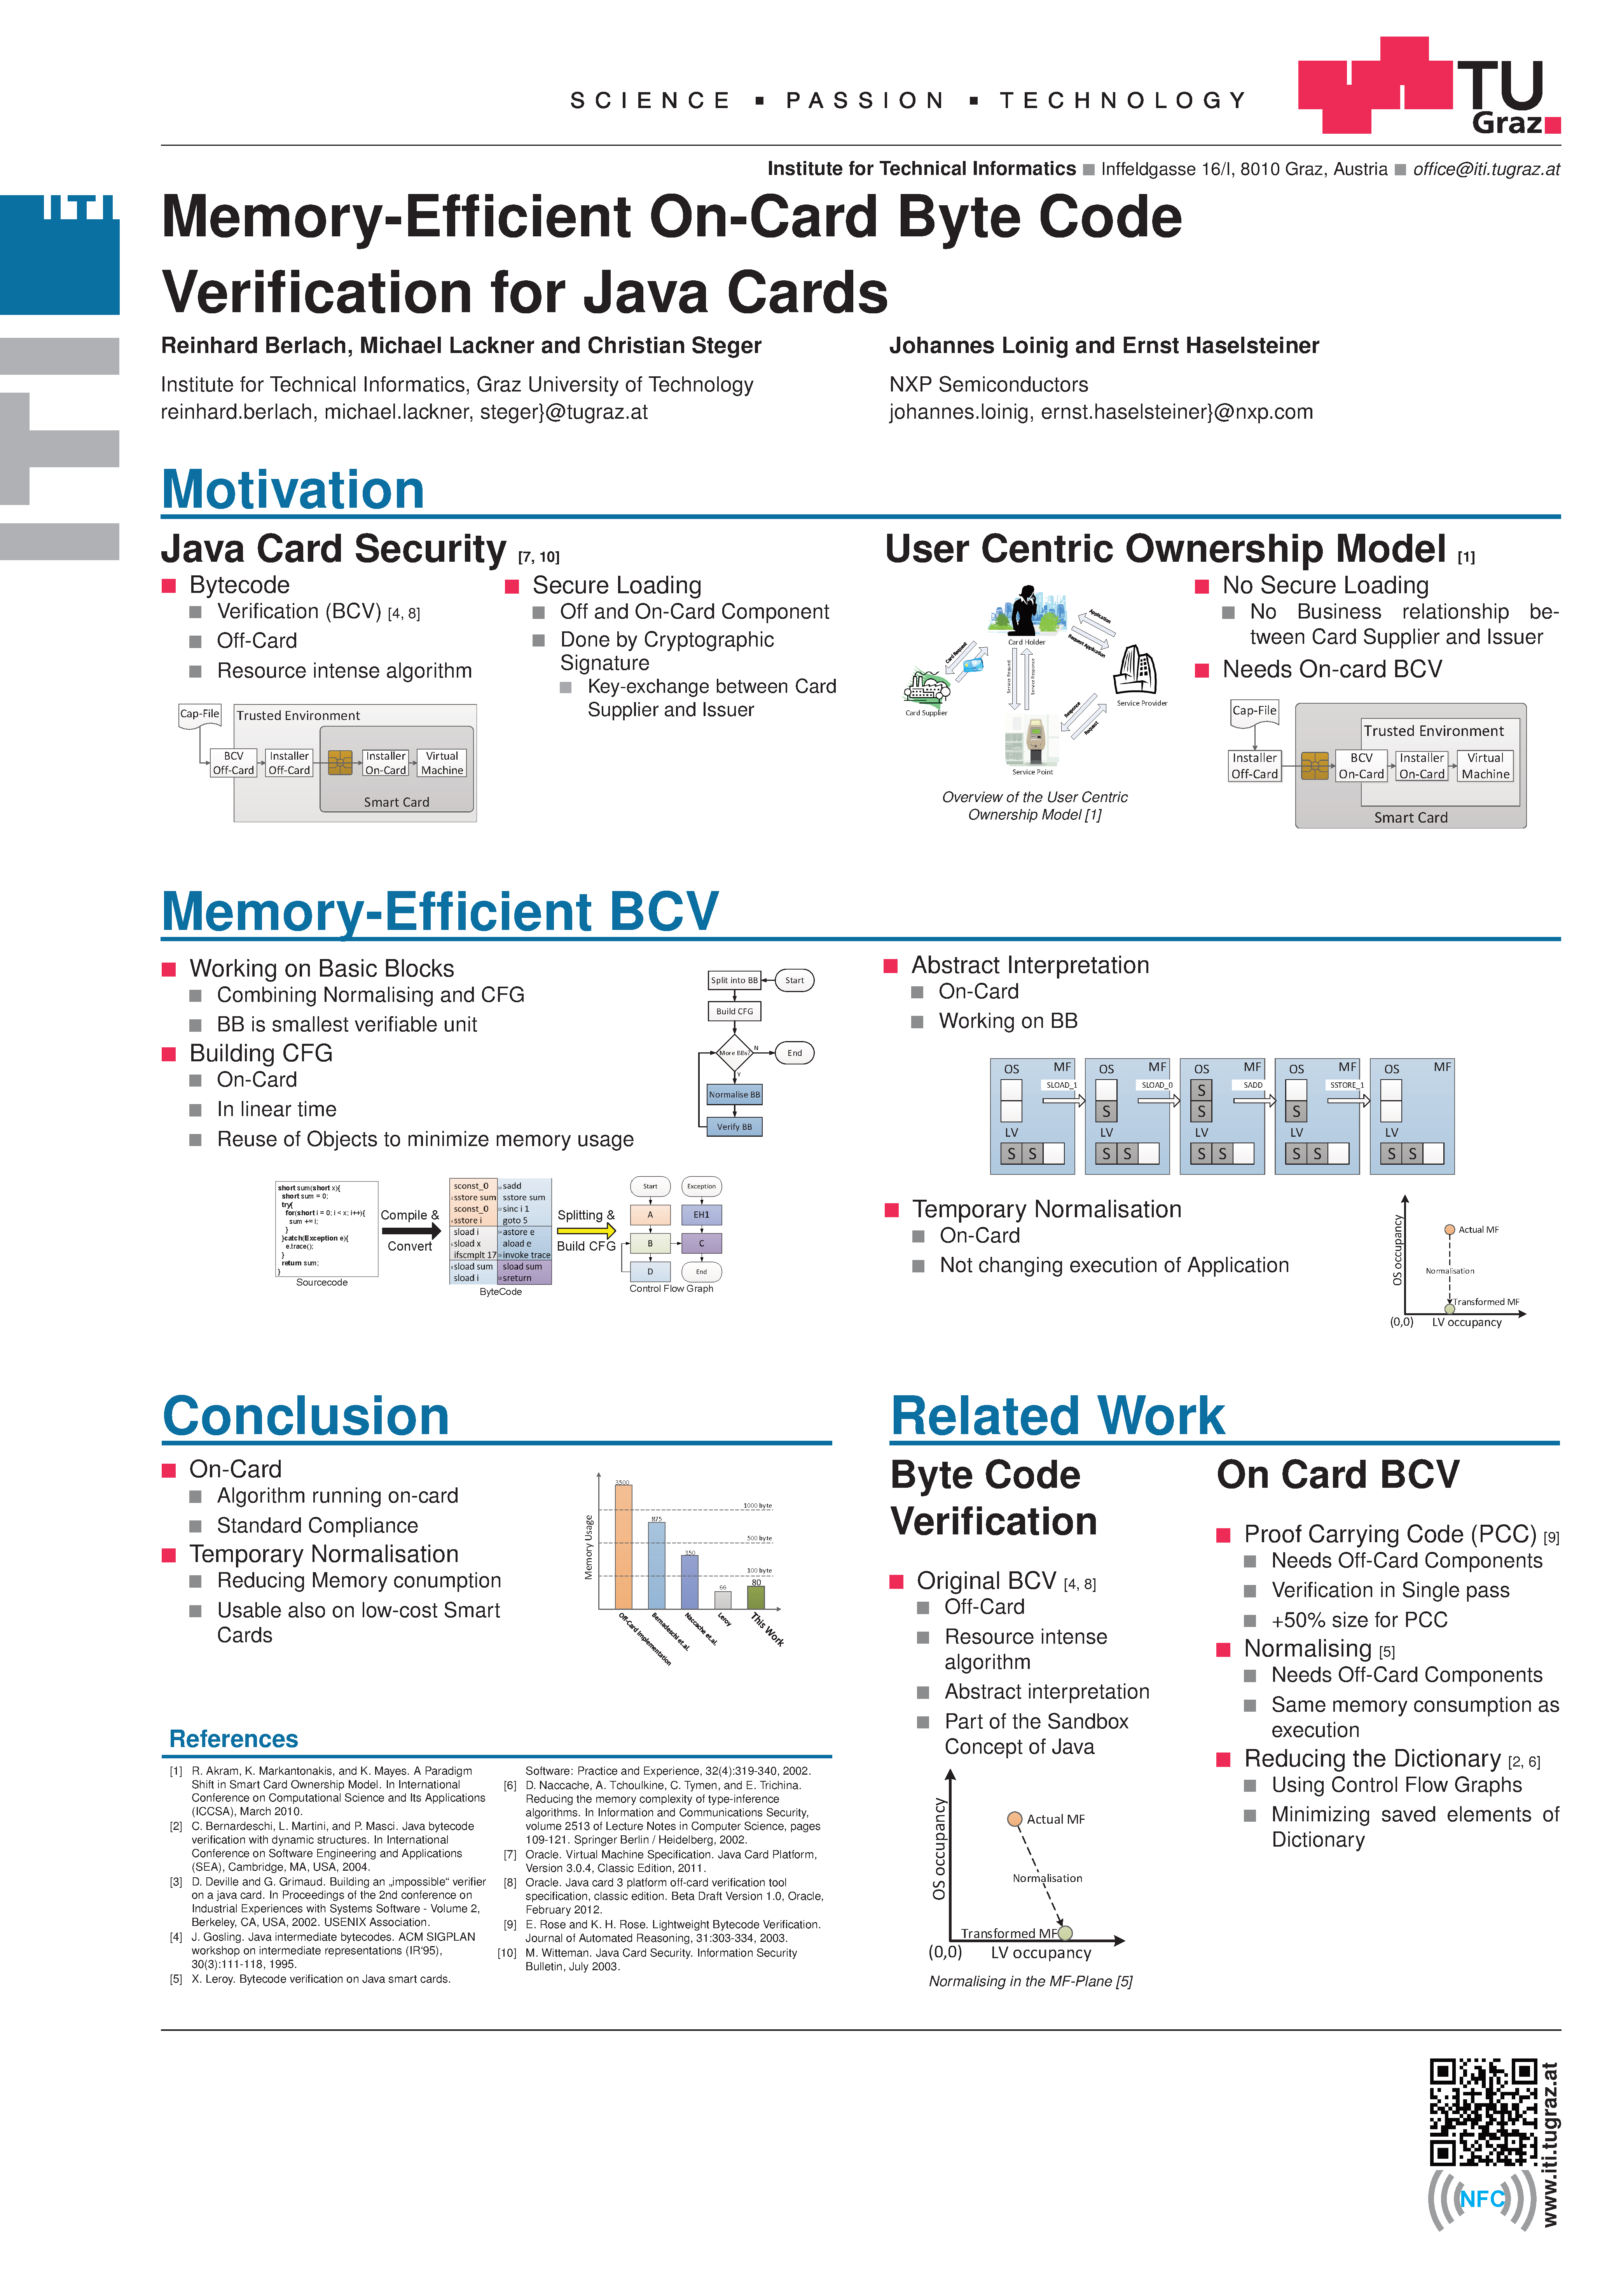
\includegraphics[width=0.8\textwidth]{sample_poster_ITI}}
\caption{Sample poster created with \tugPoster{} showing a fancy layout.}
\label{fig:sample_poster1}
\end{figure}

\begin{figure}
\centering
% \vskip1em
\fbox{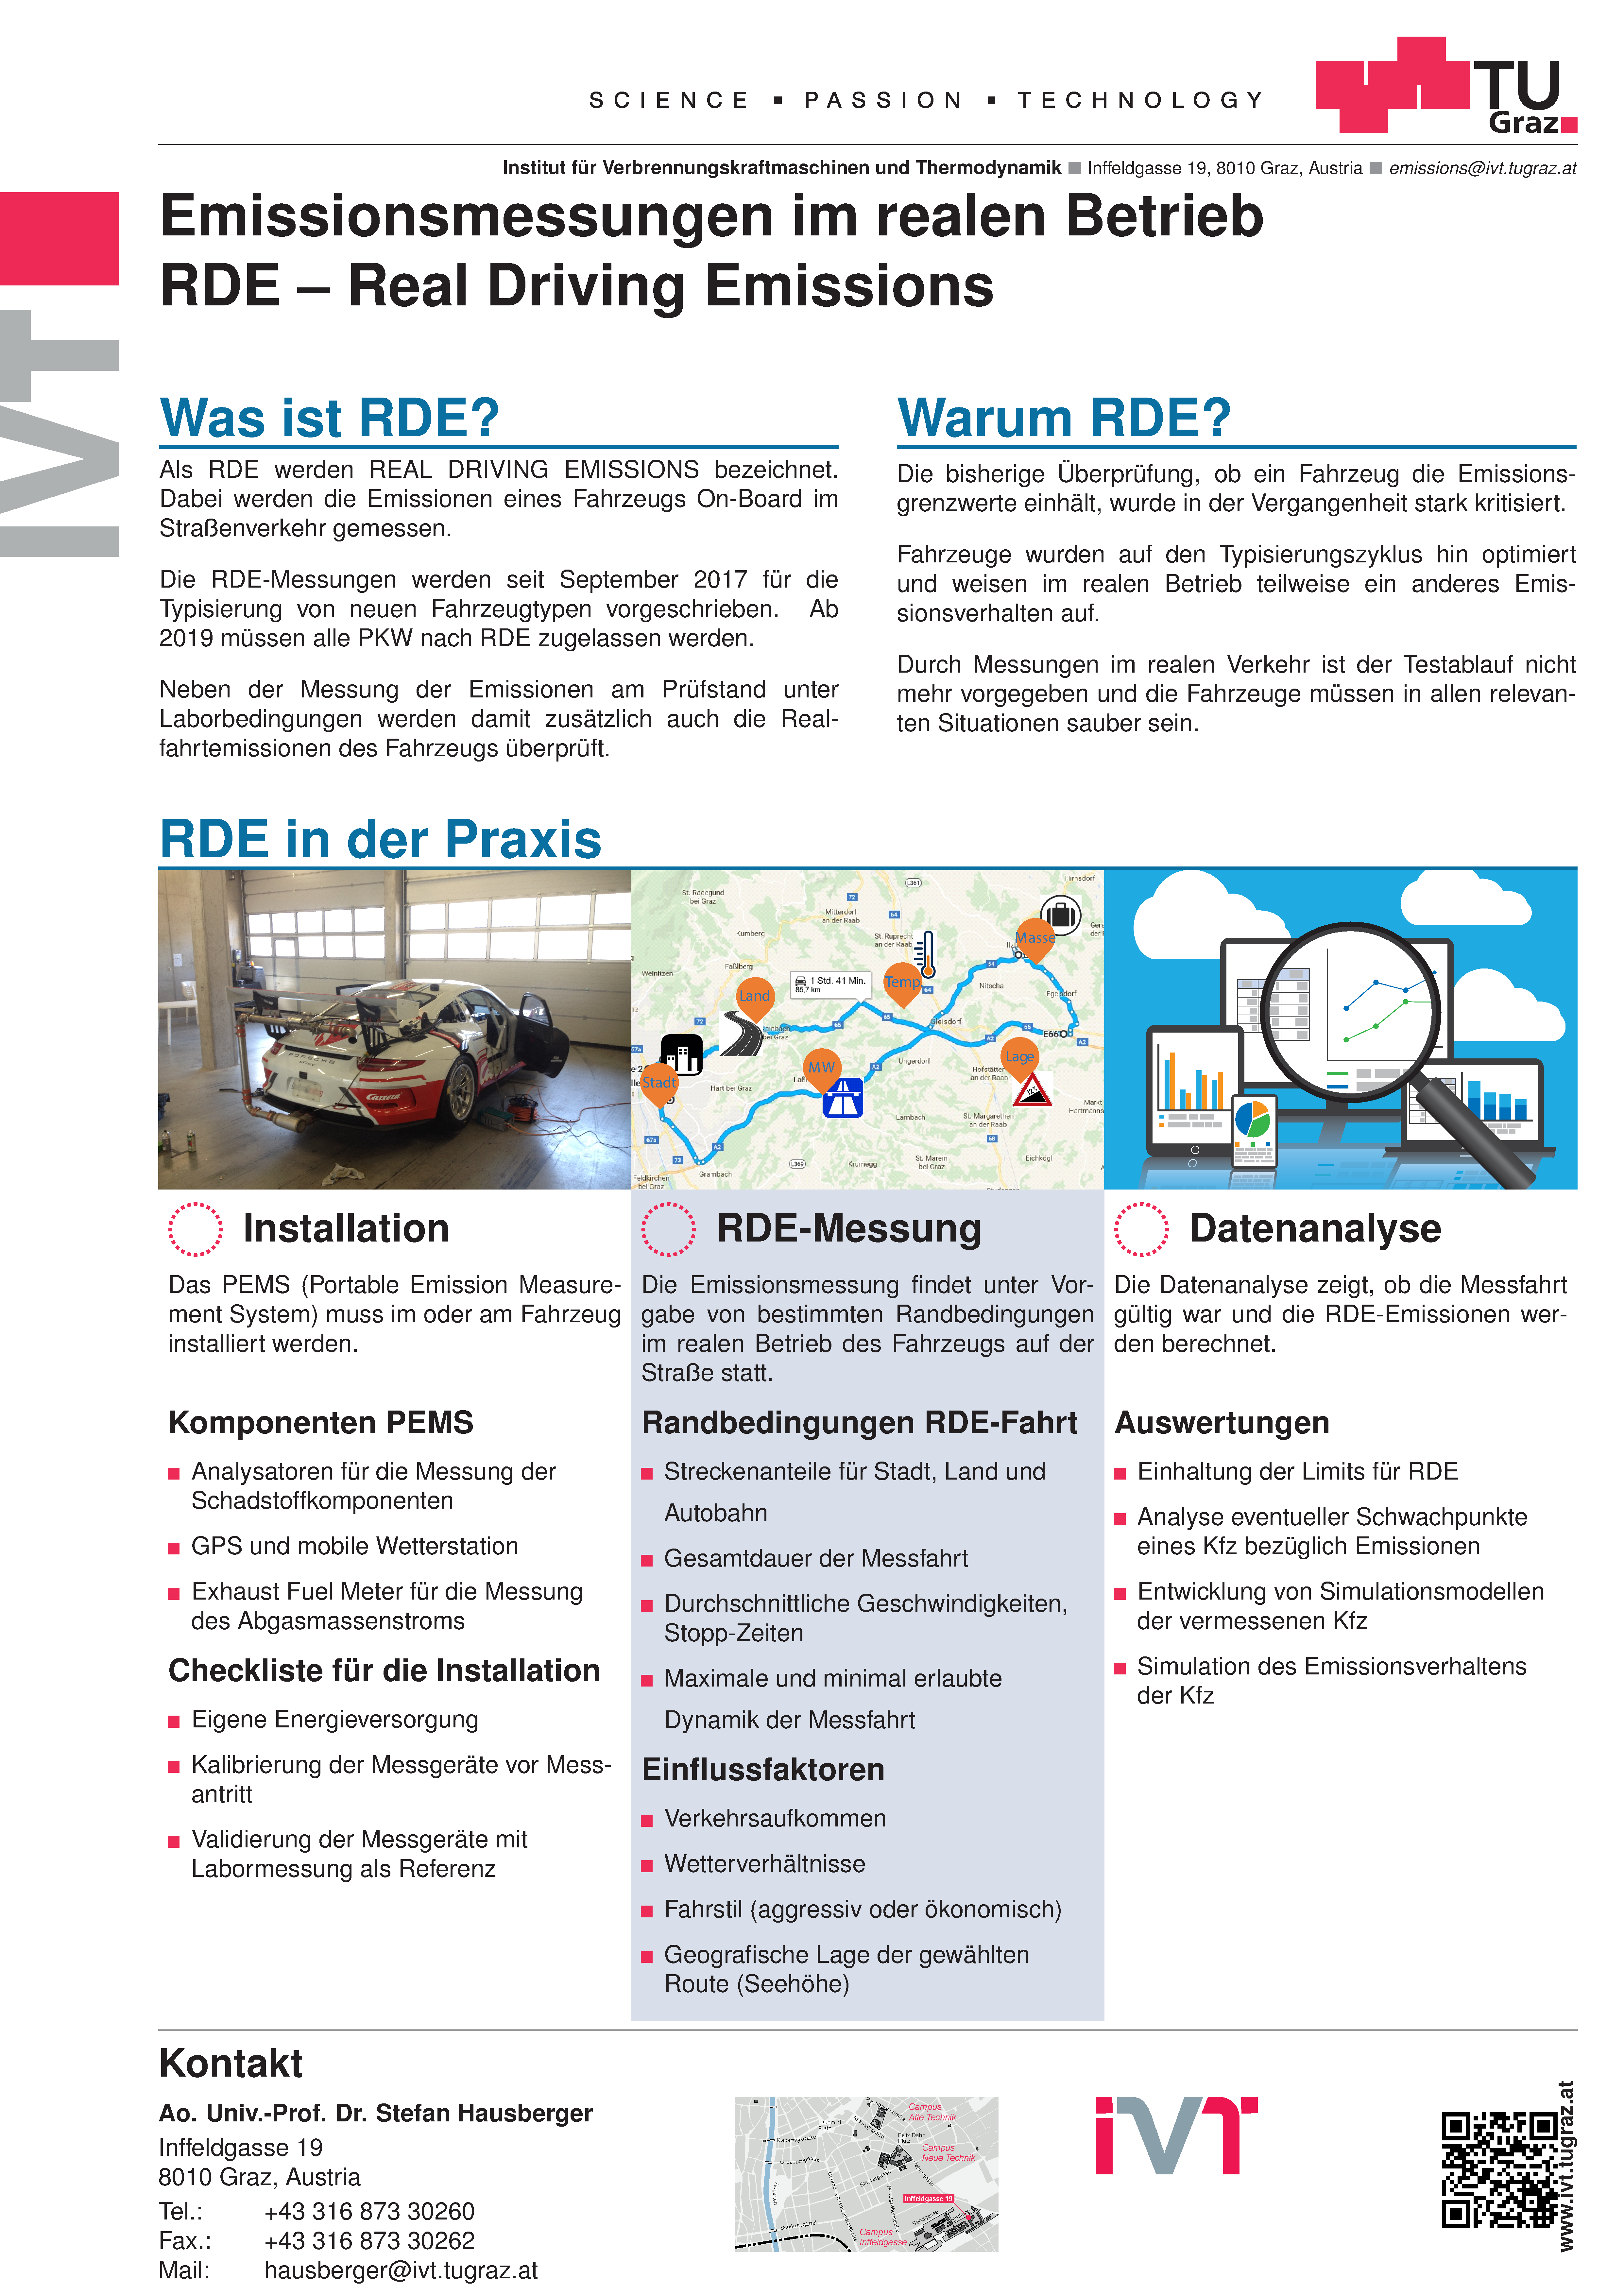
\includegraphics[width=0.8\textwidth]{sample_poster_IVT}}
\caption{Sample poster created with \tugPoster{} showing a fancy layout.}
\label{fig:sample_poster2}
\end{figure}
% \end{minipage}

\section{Debugging / Layout Support}
\label{sec:debugging}

If you need to find out why a certain content element does not move further up or to the left/right it is often helpful to show the bounding boxes of the content elements. This can be achieved by adding the class option \texttt{debug} which shows the bounding box of every content element as well as the gaps between columns.
\texttt{IPTtwocol} is shown in red, \texttt{IPTcols} is shown in green, and figures are shown in magenta (see \Cref{fig:debug}).


% \begin{minipage}{\textwidth}
\begin{figure}
\centering
\vskip1em
\fbox{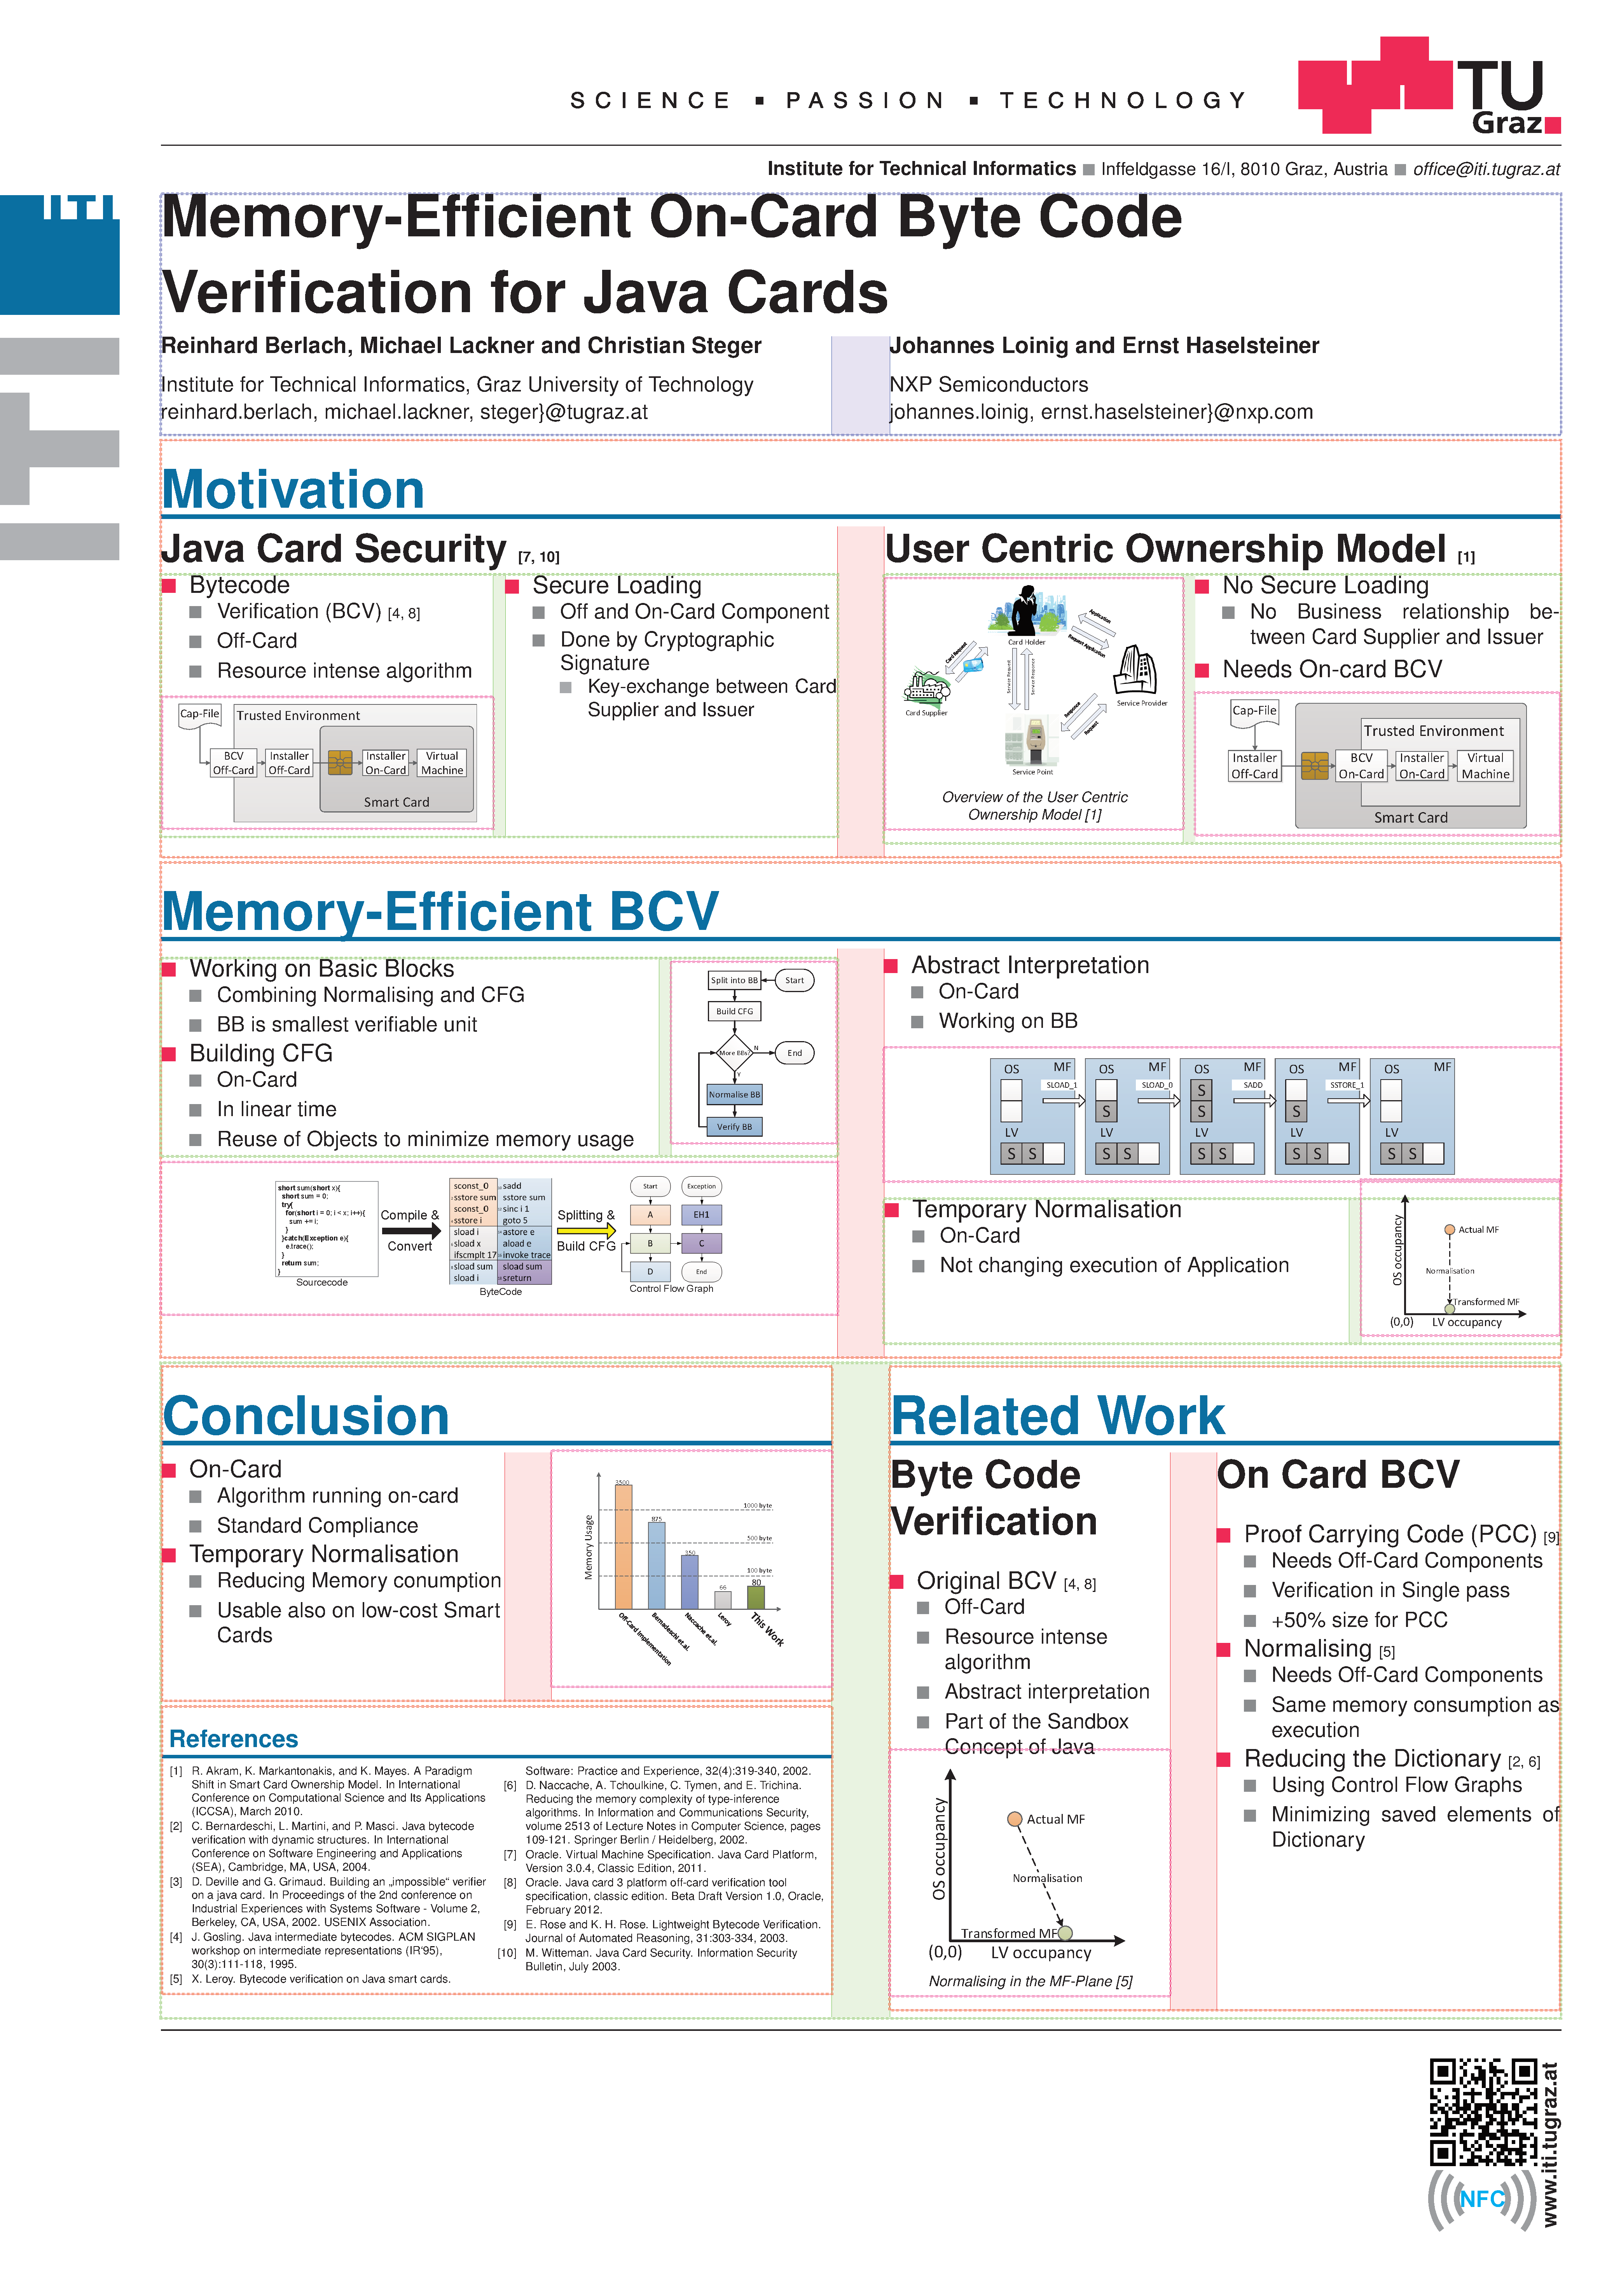
\includegraphics[width=0.8\textwidth]{sample_debug}}
\caption{Sample poster with the \texttt{debug} option enabled.}
\label{fig:debug}
\end{figure}
% \end{minipage}

\begin{figure}
\centering
\vskip1em
\fbox{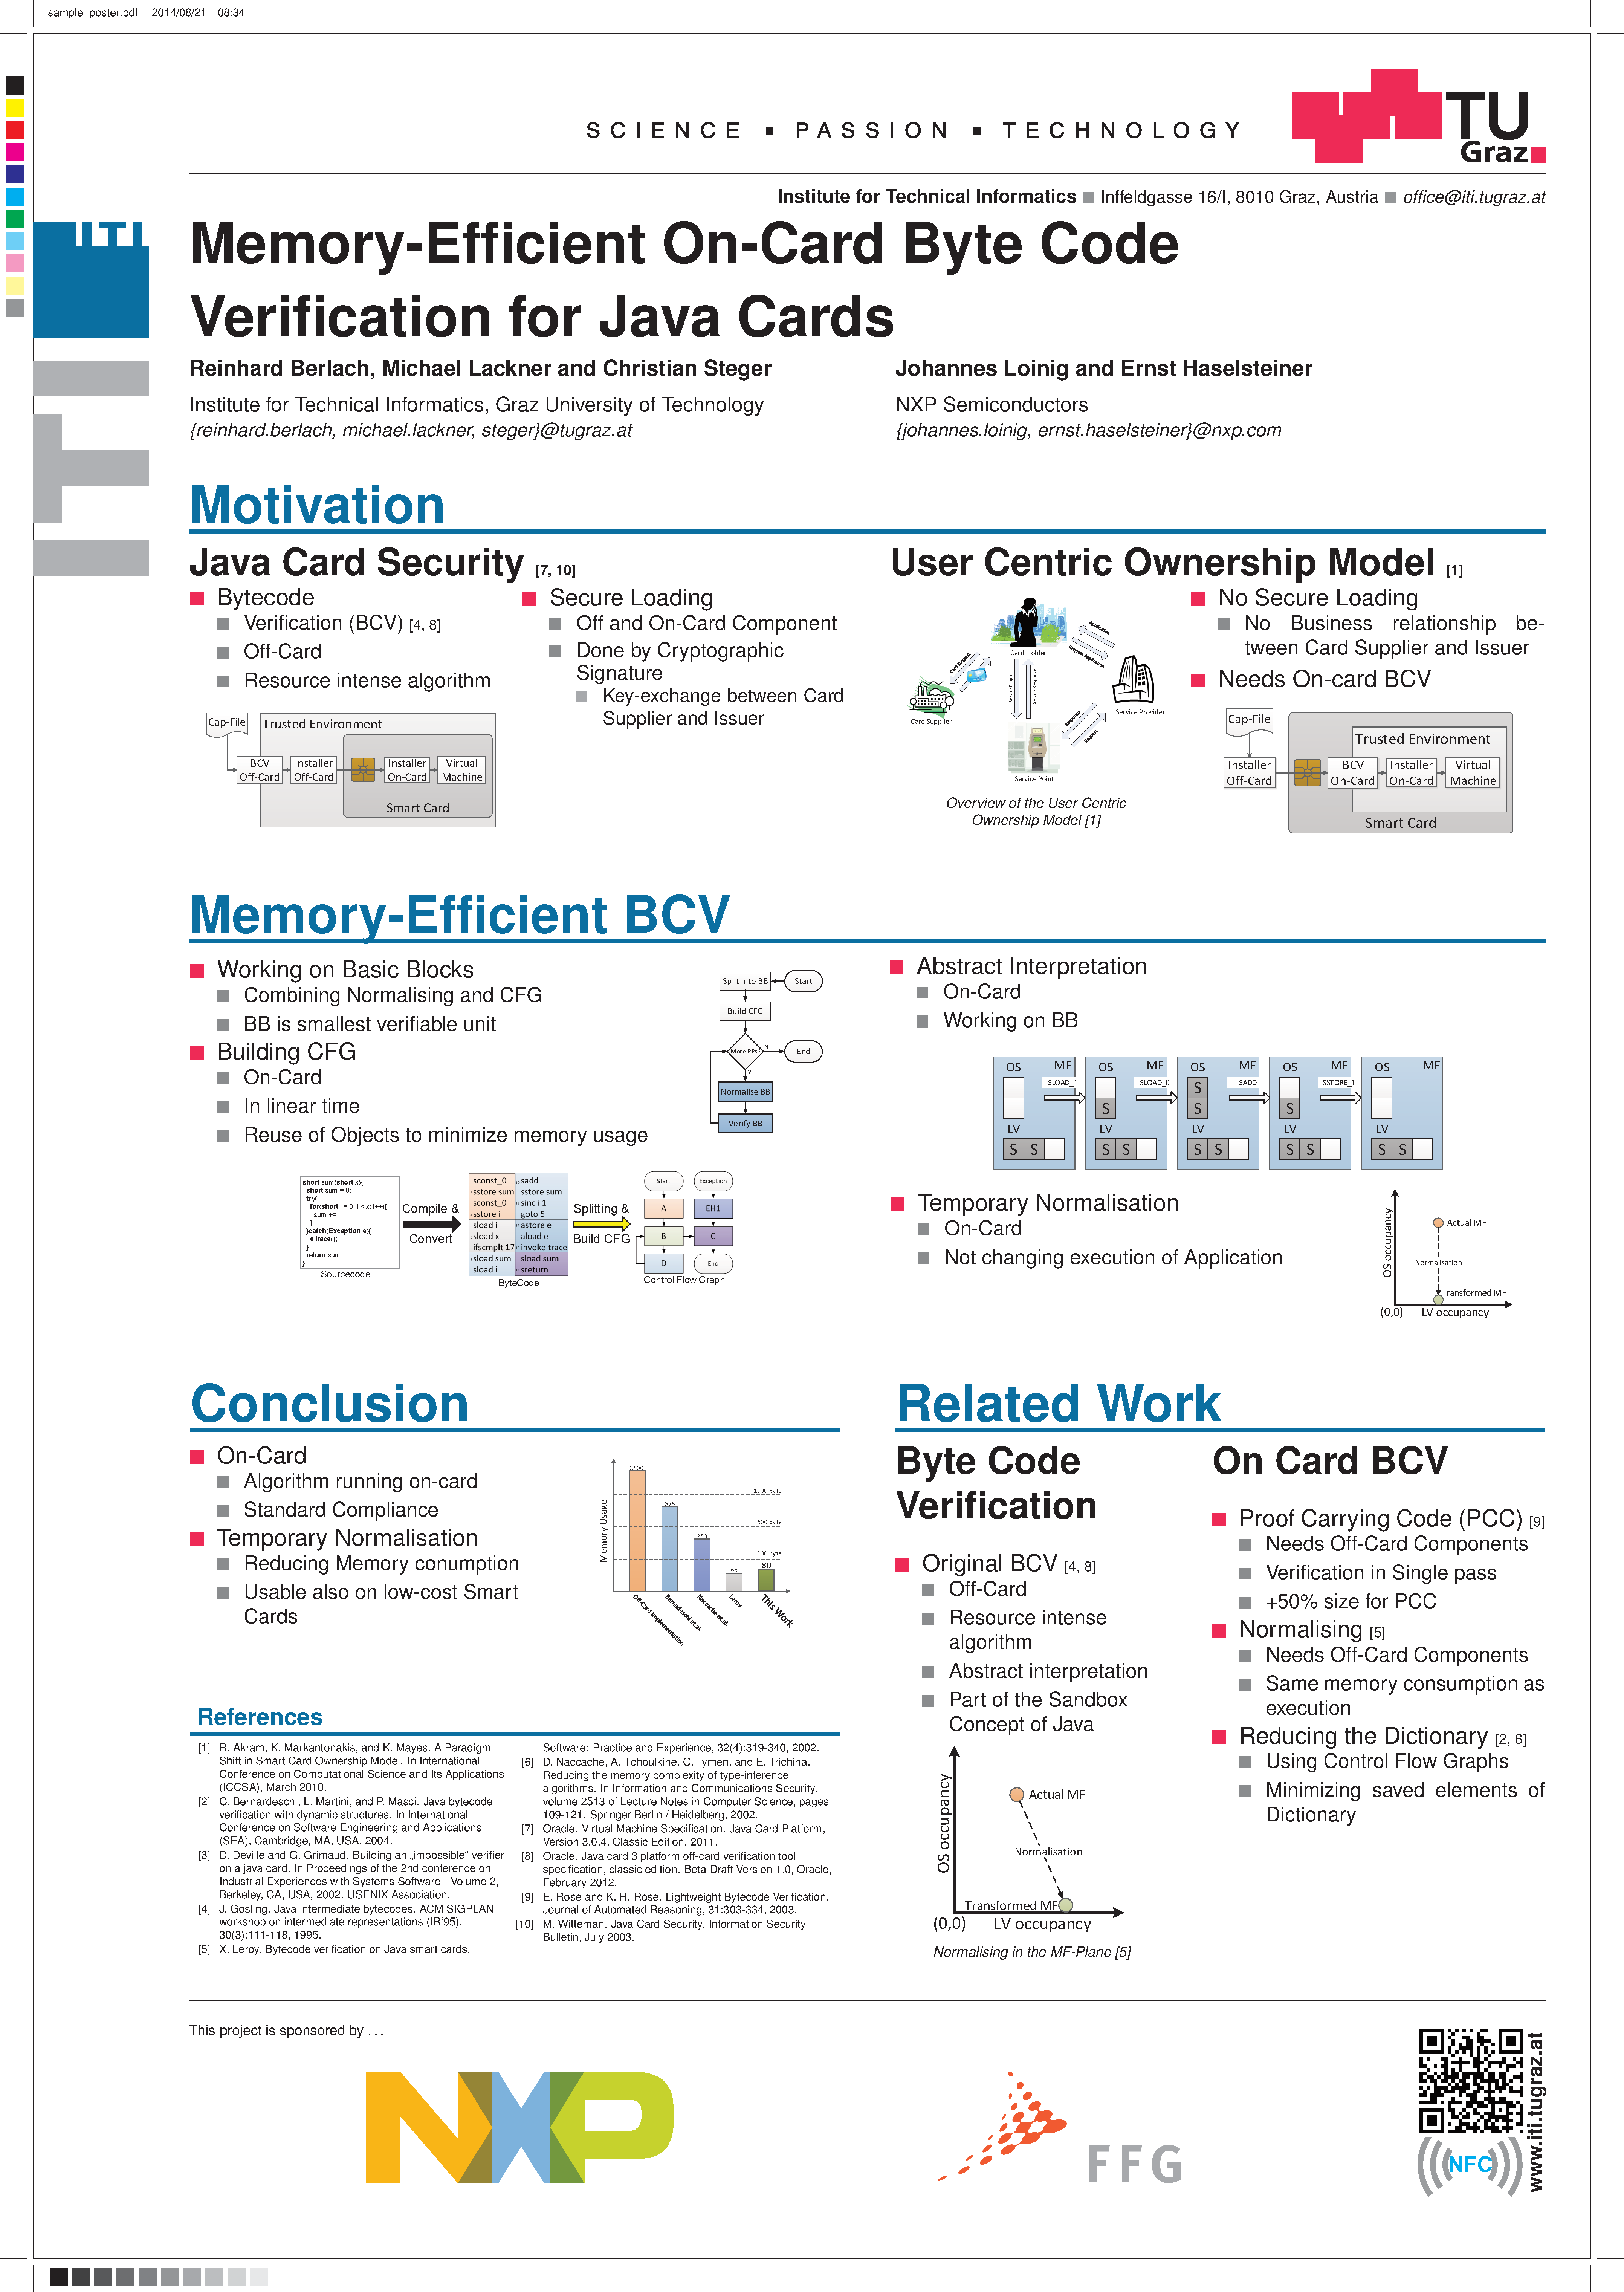
\includegraphics[width=0.8\textwidth]{sample_cropmarks}}
\caption{Sample poster with a ``crop rectangle'' ready to print and easy cutting.}
\label{fig:cropmarks}
\end{figure}

\section{Known Issues}

Currently there are no known issues. But in case you find some ``misbehavior'' feel free to contact the author with a detailed description ;-)

It would be nice to integrate bibtex for generating the references automatically. Maybe this will be added in a future version.

\end{document}